\documentclass{article}


\usepackage[backend=bibtex, style=ieee]{biblatex}
\usepackage{graphicx}
\usepackage{hyperref}
\usepackage{siunitx}
\usepackage[table]{xcolor}


\bibliography{report}
\title{Human silhouette segmentation in unconstrained videos}
\author{Miroslav Vitkov \\ sir.vorac@gmail.com}


\begin{document}
\maketitle


\begin{abstract}
Gait is a prominent biometric with similar importance to face recognition.
It is feasible in the presence of heavy noise like darkness or low quality cameras.
The input to the recogniser algorithm is usually a segmented and deshadowed human silhouette.
This report presents an implementation of the segmentation step.
We use Histogram of Oriented Gradients for dimensionality reduction and a Support Vector Machine for detection followed by approximate median filter for segmentation.
\end{abstract}


\section{Introduction}
\subsection{Gait}
The interdisciplinary field of human identification via gait is now 42 years old.
Initially, glowing markers were used\cite{begin} for 38\% recognition accuracy, compared to random chance of 16.7\%.

Further development split into model-free and model-based methods.
Model-free methods look at pixels, one notable work being the gait energy model\cite{energy}.
Model-based approaches use a strong prior, e.g. a pendulum model of legs\cite{pendulum}.

Modern methods are dominated by motion vector estimated approaches, such as \cite{pyramid}
A recent improvement to \cite{pyramid} demonstrates human recognition accuracy of 96\% using a fusion of a visible spectrum camera, a Microsoft Kinetic and a wearable accelerometer\cite{robust}.


\subsection{Silhouette}
One common preprocessing step is adaptively threshold background subtraction \cite{vehicle}.
Pixels in consecutive frames are compared and if the difference is less that a threshold value, classified as background and thus not interesting.
The threshold is generated by an exponential filter.
The difference is computed by sum of absolute difference (SAD) \cite{background}.
This allows the procedure to ignore periodic noise e.g waving tree leaves and low-frequency noise e.g. parked car or change of illumination level.

The Histograms of Oriented Gradients (HOG)\cite{hog} descriptor encodes an an image's local colour gradients.
It works in a sliding window or square or circular shape.
Horizontal and vertical derivatives are calculated with a centered mask (1 0 1).
All generated values in the window are summarised into one tuple (direction, magnitude).
This approach is believed to work better than the earlier Local Binary Patterns.


\section{Dataset}
\subsection{What is out there}
Numerous human tracking outdoor datasets are described in the literature\cite{datasets0}\cite{datasets1}.
Notable is the occlusion dataset\cite{datasets2}, providing experience close to real world outdoor surveillance.
Also the AVA indoor dataset\cite{ava} consists of a large number (1200) single view videos.

\subsection{What was chosen}
The best siloutette segmentation dataset seems to be Supervisely's human dataset\cite{supervisely}. This is a sample from it:
\\
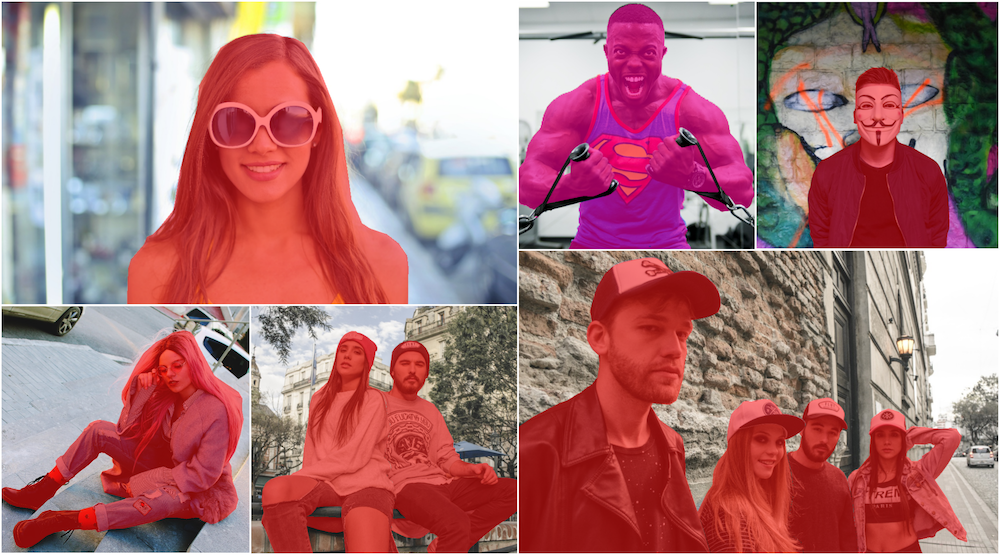
\includegraphics[height=0.5\textwidth]{../img/supervisely}
\\
compare it to COCO's segmented siloutettes:
\\
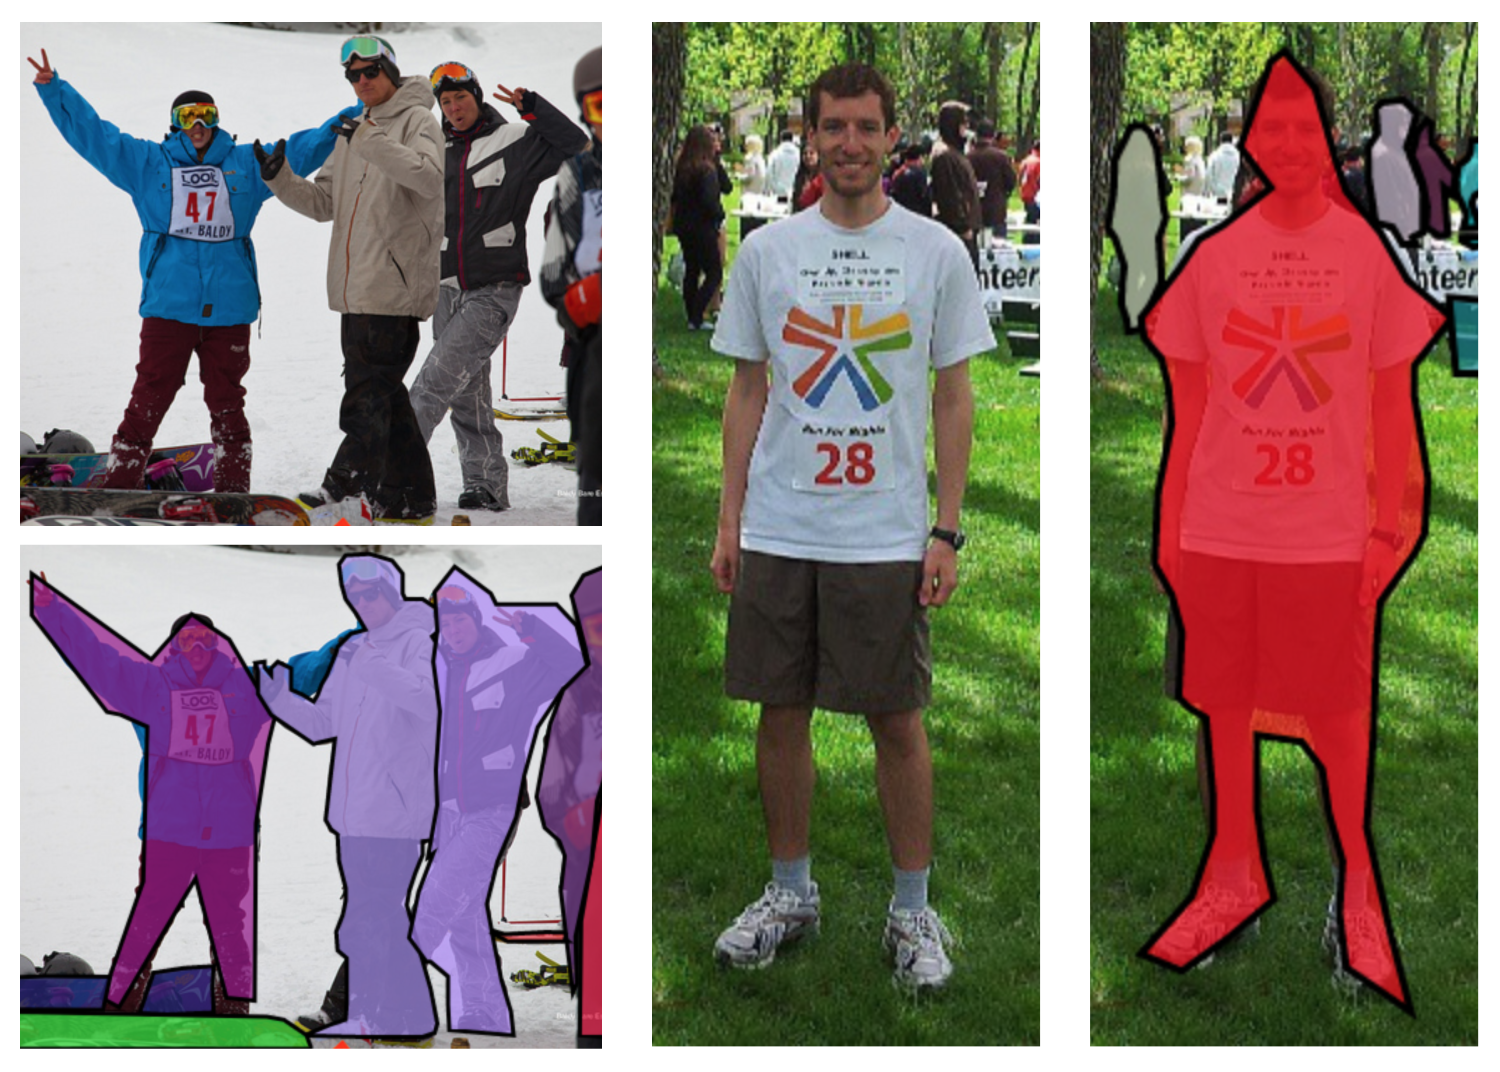
\includegraphics[height=0.5\textheight]{../img/coco}.

\subsection{In addition to that}
Segmenting silouettes by static images is increadibly difficult.
To fasciliate the task, a dataset of videos was compiled.
It was expected to fasciliate frame-to-frame adaptive background subtraction in preselected regions to generate the actual silouettes.
It consists of X videos of a single walking subject, totalling S seconds of footage.


\section{Method}
Train the detector:
\begin{enumerate}
\item{Process one frame at a time.}
\item{Choose a number P of positive training examples and a number N of negative examples. Let N>>P. Also let N + P be as large as computing power is available.}
\item{Train an SVM over the HOG descriptors of the samples.}
\item{Apply hard-negative mining. That is, for slide a window across negative examples. Out of any window which produces a false positive, create an individual negative instance.}
\item{Retrain. If the gain in accuracy is substantial, repeat the previous and this step.}
\end{enumerate}

Test the detector:
\begin{enumerate}
\item{Process one frame at a time.}
\item{Run the model on a sliding window at various scales and positions.}
\item{Apply non-negative suppression on detected bounding boxes.}
\end{enumerate}

Segmentation:
\begin{enumerate}
\item{Work on the whole video.}
\item{Perform foreground segmentation by approximate median filter\cite{amf}}
\item{Run the detector on any blobs of foreground.}
\item{For every detected bounding box, consider all foreground pixels inside to be a human silhouette.}
\item{Test the complete algorithm on a small hand-crafted dataset.}
\end{enumerate}


\section{Results}
To be released.
Same for the implementation.


\printbibliography


\end{document}

